\section{Konzept}
Hier wird ein Konzept mit Mock Ups und Architektur entstehen

\subsection{Priorisierung der Erfassungsmöglichkeiten}
\subsectionauthor{Lukas Seemann}
Im Anschluss an die Auswahl der Erfassungsmöglichkeiten werden diese Möglichkeiten nun priorisiert. In der folgenden Tabelle (Tabelle 1) ist die Priosierung abgebildet. \newline
\begin{table}[h]
	\centering
	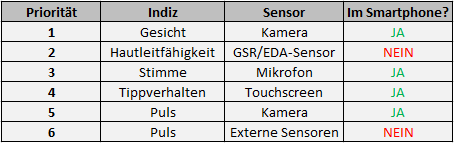
\includegraphics[width=14cm]{Bilder/prio.png}
	\caption[Priorisierung der Erfassungsmöglichkeiten]{Priorisierung der Erfassungsmöglichkeiten}
\end{table}%
\newline In der ersten Spalte ist die Priorität dargestellt. Je niedriger die Zahl ist, desto höher ist die Erfassungsmöglichkeit priorisiert. Die Möglichkeiten werden in der Reihenfolge der hier dargestellten Priorisierung thematisiert und letzten Endes in den Prototyp der mobilen Applikation integriert, um Daten zu erfassen. Je nachdem wie viel Zeit die einzelnen Features benötigen, können mehr und mehr Möglichkeiten der Datenerfassung in die App eingebaut werden, wenn sie noch im Zeitrahmen der Studienarbeit umsetzbar sind. Bei den einzelnen Möglichkeiten werden das Indiz, anhand dessen Rückschlüsse auf eine Emotion gemacht werden kann, und ein Sensor, der Daten zum Indiz für die App erfassen soll, aufgelistet. In der letzen Spalte ist festgehalten, ob der benötigte Sensor in den meisten aktuellen Smartphones bereits enthalten ist oder nicht. \newline
Die höchste Priorität hat das Indiz der Hautleitfähigkeit, die mithilfe von GSR- beziehungsweise EDA-Sensoren erfasst werden kann. Diese Art von Sensoren befinden sich nicht in handelsüblichen Smartphones, weshalb man hierzu externe Sensoren mit dem Handy verbinden muss. \newline
...

\subsection{Übertragung biometrischer Daten in Indikatorscores}
\subsectionauthor{Lukas Seemann}
Die von den Smartphone-internen und externen Sensoren zurückgeliefert Daten müssen in der App einheitlich verarbeitet werden. Die zurückgelieferten Daten sind unterschiedlich und meistens selbst nicht aussagend. Mit dem im Theorieteil erklärten Hintergrundwissen ist es jedoch möglich, die Daten zu interpretieren. \newline 
Im Umfeld der App soll diese Interpretation mithilfe von Indikatoren geschehen. Ein Indikator ist in diesem Kontext ein Anzeichen, das für die Emotionsbestimmung herangezogen werden kann. Es existieren einerseits Indikatoren, die sich nur für die Bestimmung einer Emotion eignen, und andererseits auch Indikatoren, die für mehrere Emotionen ausschlaggebend sind. Folgende Indikatoren sind für die Umsetzung geplant: 
\begin{itemize}[noitemsep, topsep=0pt]
	\item stress,
	\item happyIndicator,
	\item sadIndicator,
    \item angryIndicator und
    \item suprisedIndicator.
\end{itemize}
In Abbildung ? ist der Ablauf der Bestimmung von Indikatorscores abbgebildet. Unabängig davon, welcher Sensor verwendet wird, seine Daten müssen immer auf diese Indikatoren abgebildet werden. Für jeden Sensor muss dabei ein Bereich bestimmt werden, wann immer eine neue Auswertung der Sensordaten zu den sogenannten Indikatorscores geschieht. Eine Auswertung kann generell dann durchgeführt werden, wenn genug Daten vorhanden sind, die aussagekräftig für die Indikatoren sind. Dies ist von Sensor zu Sensor unterschiedlich und muss dementsprechend berücksichitgt werden. \newline
Bei einer Auswertung werden die einzelnen Indikatoren mit Scores von null bis eins versehen, sodass man pro Auswertung der Sensordaten mehrere Indikatorscores erhält. Die Logik für das Setzen der Indikatorscores muss mithilfe von Mappern umgesetzt werden. Für jeden Sensor muss dafür ein individueller Mapper existieren. Die Mapper werden immer dann aufgerufen, wenn genügend Daten des Sensors vorhanden sind. \newline
\begin{figure}[h]
	\centering
	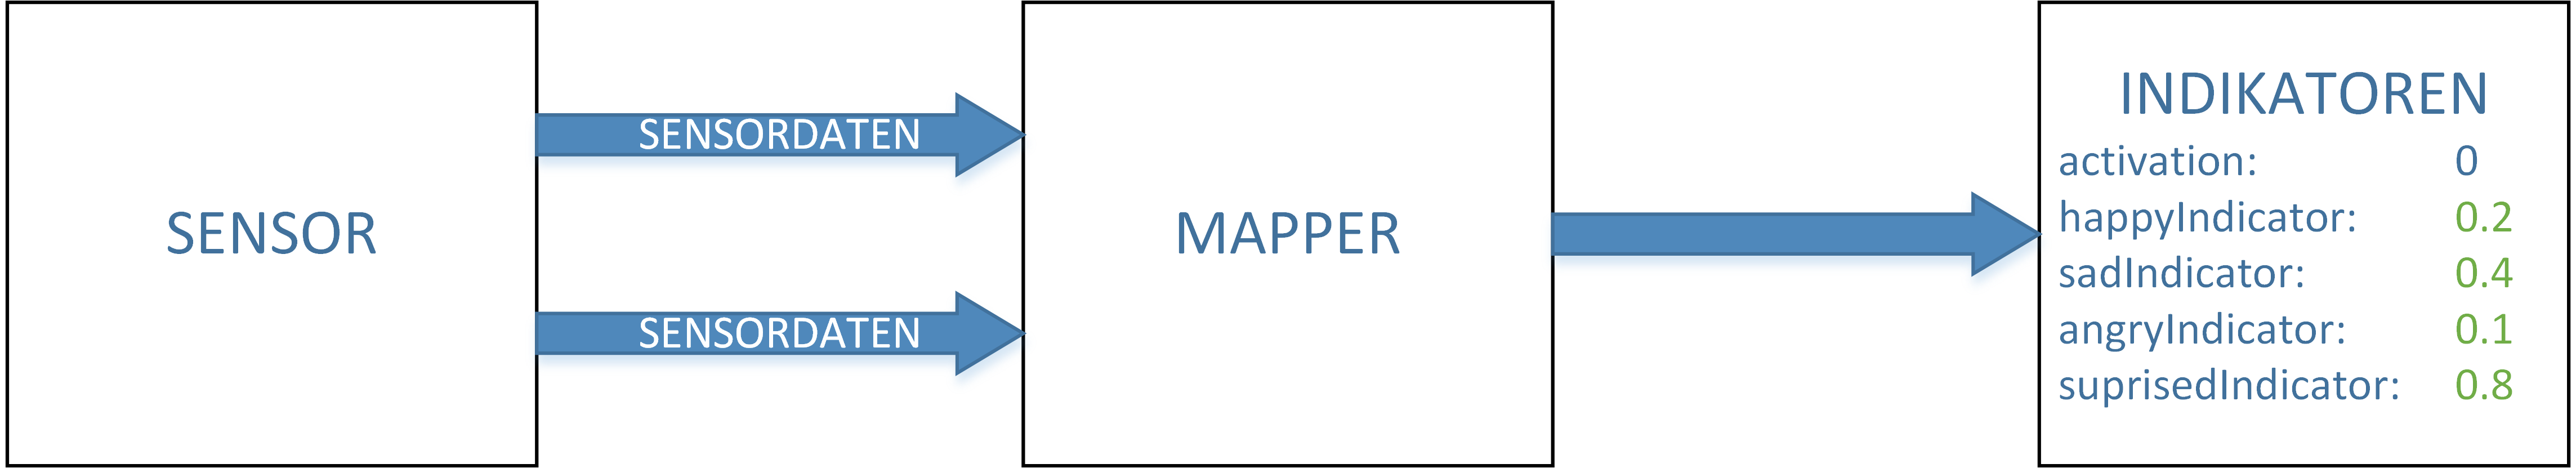
\includegraphics[width=16cm]{Bilder/indicatorscore.png}
	\caption[Ablauf der Erstellung von Indikatorscores]{Ablauf der Erstellung von Indikatorscores}
\end{figure}%
\subsection{Auswertung der Indikatorscores zur Emotionsbestimmung}
\subsectionauthor{Lukas Seemann}
Aus den angesammelten Indikatorscores muss nun entschieden werden, welche Emotion am wahrscheinlichsten beim Benutzer der App vorliegt. Diese Auswertung der Indikatorscores zu konkreten Emotionen lässt sich in zwei Bestandteile aufteilen: die Menge der Kausalitätsregeln und den Entscheidungsalgorithmus. Als Ergebnis wird pro Emotion ein Emotionscore erwartet, der angibt, inwiefern die Emotion beim User zum getesteten Zeitpunkt vorliegt.
\subsubsection{Kausalitätsregeln}
\subsubsectionauthor{Lukas Seemann}
Eine Kausalitätsregel erwartet eine Menge von Indikatorscores als Eingabe und wendet basierend auf den Indikatorscores Effekte auf die vorhandenen Emotionscores an. Die Indikatoren werden also je nach ihren Werten in verschiedene Emotionen übersetzt. \newline Eine Kausalitätsregel besteht immer aus einer Bedingung und einer Score-Transformation. Eine Bedingung betrifft einen oder maximal zwei Indikatorscores und legt fest, wann die Score-Transformation der Kausalitätsregel ausgeführt wird. Die Score-Transformation beschreibt Effekte, die auf die Emotionscores angewandt werden. Beispielsweise würde einer hoher Score des Stress-Indikators zu positiven Effekten für die Emotionen happy, angry und suprised führen. In Abbildung ? ist der Ablauf der Ausführung einer solchen Kausalitätsregeln gezeigt. Die Formulierung von realitätsgetreuen Kausalitätsregeln ist ausschlaggebend dafür, wie präzise die Anwendung letzten Endes die Emotionen bestimmmen kann. \newline
\begin{figure}[h]
	\centering
	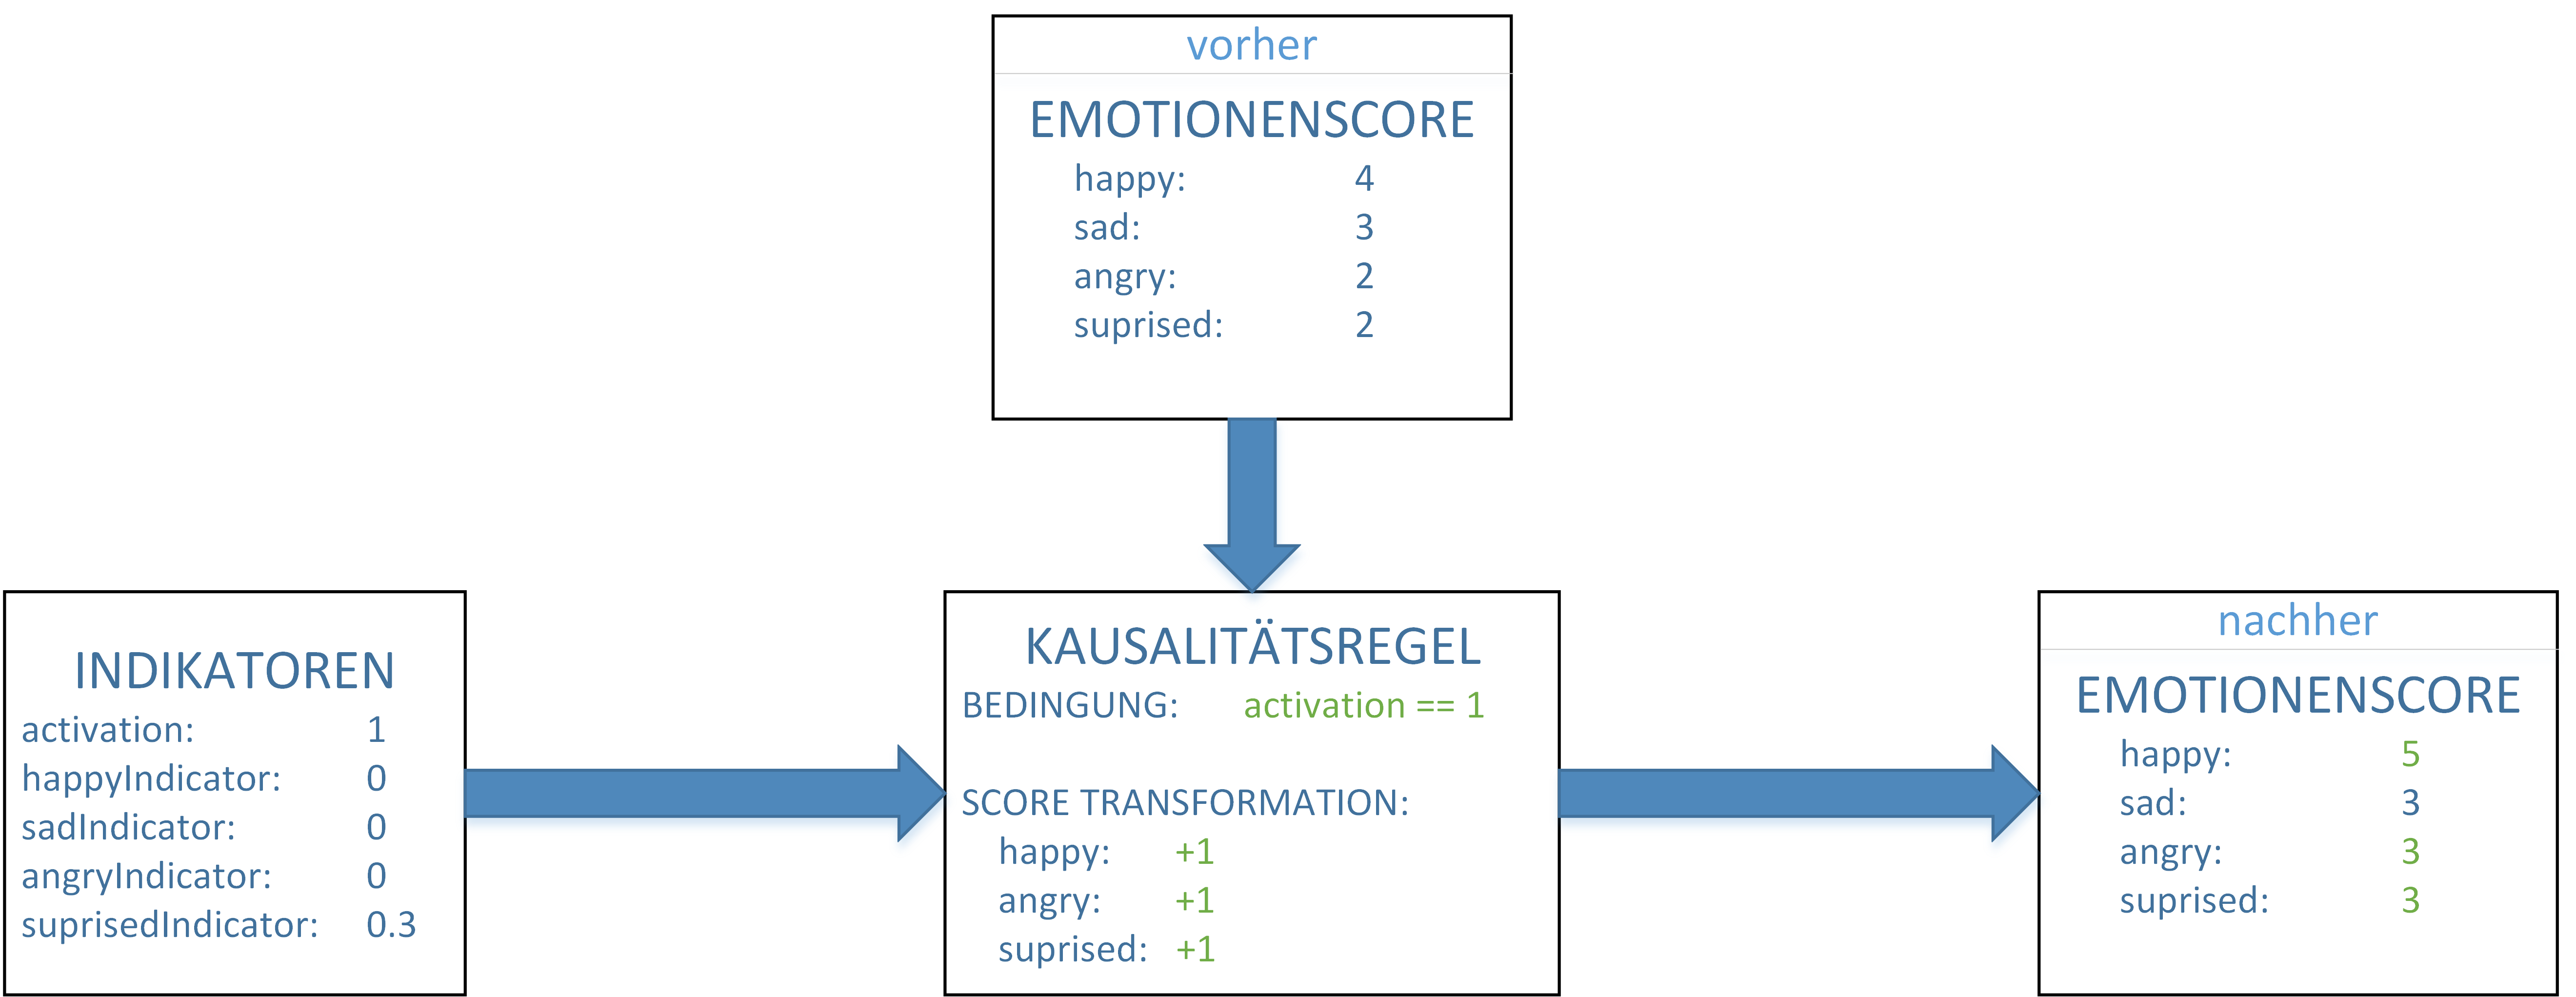
\includegraphics[width=16cm]{Bilder/causalityrules.png}
	\caption[Ablauf der Ausführung von Kausalitätsregeln]{Ablauf der Ausführung von Kausalitätsregeln}
\end{figure}%
\subsubsection{Entscheidungsalgorithmus}
\subsubsectionauthor{Torben Brenner}
Ziel der Anwendung ist es, basierend auf zuvor aufgenommenen Daten eine Entscheidung zu fällen, welche Emotion der Nutzer der 
Anwendung aktuell empfinden könnte. Die Entscheidung muss dabei die verschiedenen Ergebnisse der Auswertungsebene einbeziehen
und aus diesen auf eine Emotion schließen. Deshalb muss eine Einheitliche Datenstruktur entwickelt werden, über die die Auswertungsebene
die Daten zur Verfügung stellt. \\
Die Entscheidung könnte hierbei über ein \textit{Scoring} entstehen. Dieses \textit{Scoring} müsste dabei auf der Auswertungsebene stattfinden, 
wobei jeder der Auswertungsalgorithmen ein \textit{Scoring} für die verschiedenen Emotionen angeben muss. Am Ende könnten z. Bsp. die verschiedenen 
\textit{Scorings} addiert und die Emotion mit dem höchsten \textit{Scoring} ausgewählt werden.
\subsection{Ionic Framework}
In diesem Kapitel wird das Ionic Framework, das für die Umsetzung der mobilen Applikation verwendet wird, vorgestellt und die Gründe für die Verwendung aufgezeigt.
\subsubsection{Aufbau und Einsatz des Frameworks}
\subsubsectionauthor{Lukas Seemann}
Ionic ist ein unter der MIT License stehendes Open-Source-Framework, das zur Entwicklung von plattformübergreifenden, mobilen Applikationen dient. Mit Ionic entwickelte Apps sind damit unter anderem auf Endgeräten lauffähig, die die Betriebssysteme Android, iOS und Windows Phone benutzen. \footcite{Ion18a}
\begin{figure}[h]
	\centering
	
\includegraphics[width=11cm]{Bilder/ionic.png}
	\caption[Ionic Framework - Logo]{Ionic Framework - Logo\footnotemark}
\end{figure}%
\footcitetext{Wik18}
\newline
Aktuell befindet sich das Framework in der Version 3.9.2\footcite[Vgl. ][]{Ion18b} und befindet sich in stetiger Weiterentwicklung. Das Ionic Framework basiert wiederum auf Angular, einem Framework für die Entwicklung von Web-Applikationen. Dementsprechend nutzen Ionic-Anwendungen in der Web-Entwicklung etablierte Technologien wie HTML 5, CSS und JavaScript. \footcite[Vgl. ][]{Ion18c} Wie auch im Angular Framework, wird auch die Programmiersprache TypeScript verwendet, die auf JavaScript aufbaut, sich in der Syntax sehr stark mit JavaScript ähnelt und zusätzliche Optionen zur Typisierung von Variablen oder Funktionen anbietet. \footcite[Vgl. ][]{Til17} \newline
Ionic-Anwendungen sind im Wesentlichen normale Webanwendungen, die von jedem JavaScript-fähigen Browser ausgeführt werden können. Während mithilfe von Ionic das Frontend der Anwendung festgelegt wird, kann anschließend mit Apache Cordova die Plattformunabhängigkeit umgesetzt werden. Apache Cordova bewirkt, dass sich die Webanwendungen wie native Android-, iOS- oder Windows Phone-Applikationen anfühlen. Egal auf welcher Plattform die Ionic-Anwendung installiert wird, es wird die selbe Code-Basis verwendet. Diese wird dann vor dem Installieren von Cordova so angepasst, dass sie auf den Endgeräten ausgeführt werden können. \footcite{Ion18d}
\subsubsection{Gründe für die Verwendung}
\subsubsectionauthor{Lukas Seemann}
Das Ionic Framework bietet eine Möglichkeit mit nur einer Code-Basis, eine plattform-übergreifende Applikation zu erstellen. Dies erspart einiges an Entwicklungsaufwand, da nicht jede Plattform einzeln entwickelt werden muss. Außerdem wird einem Großteil der Smartphone-Nutzer die Nutzung der erstellten App ermöglicht und ist nicht nur für Android- oder Apple-Nutzer beschränkt. \newline
Dadurch dass Applikationen des Ionic Frameworks eigenständige Webanwendungen sind, können diese problemlos von allen Browsern interpretiert und ausgeführt. Dies ist ein großer Vorteil für das Debuggen von Code, da hierfür kein Emulator oder Endgerät verwendet werden muss. Stattdessen kann die Anwendung im Browser ausgeführt und debuggt werden. \newline
Außerdem wurden bereits in anderen Projekten und im privaten Bereiche Erfahrungen mit dem Ionic Framework gemacht, sodass keine Einarbeitung bei den Entwicklungsarbeiten notwendig ist. Dies spart wiederum Zeit, die effektiv für das Entwickeln genutzt werden kann. 
\subsection{Architektur der mobilen Applikation}
In diesem Kapitel wird die Architektur der mobilen Applikation beschrieben. Die Architektur wird in Front- und Backend der App unterteilt.
\subsubsection{Backendlogik}
\subsubsectionauthor{Lukas Seemann}
Zunächst wird explizit auf das Backend beziehungsweise die Hintergrundlogik der App eingegangen. Für das oben beschriebene Konzept bietet sich eine Umsetzung mit Javascript Klassen an, aus welchem Grund ein UML-Diagramm angefertigt werden kann. Dieses ist in Abbildung ? gezeigt. \newline
\begin{figure}[h]
	\centering
	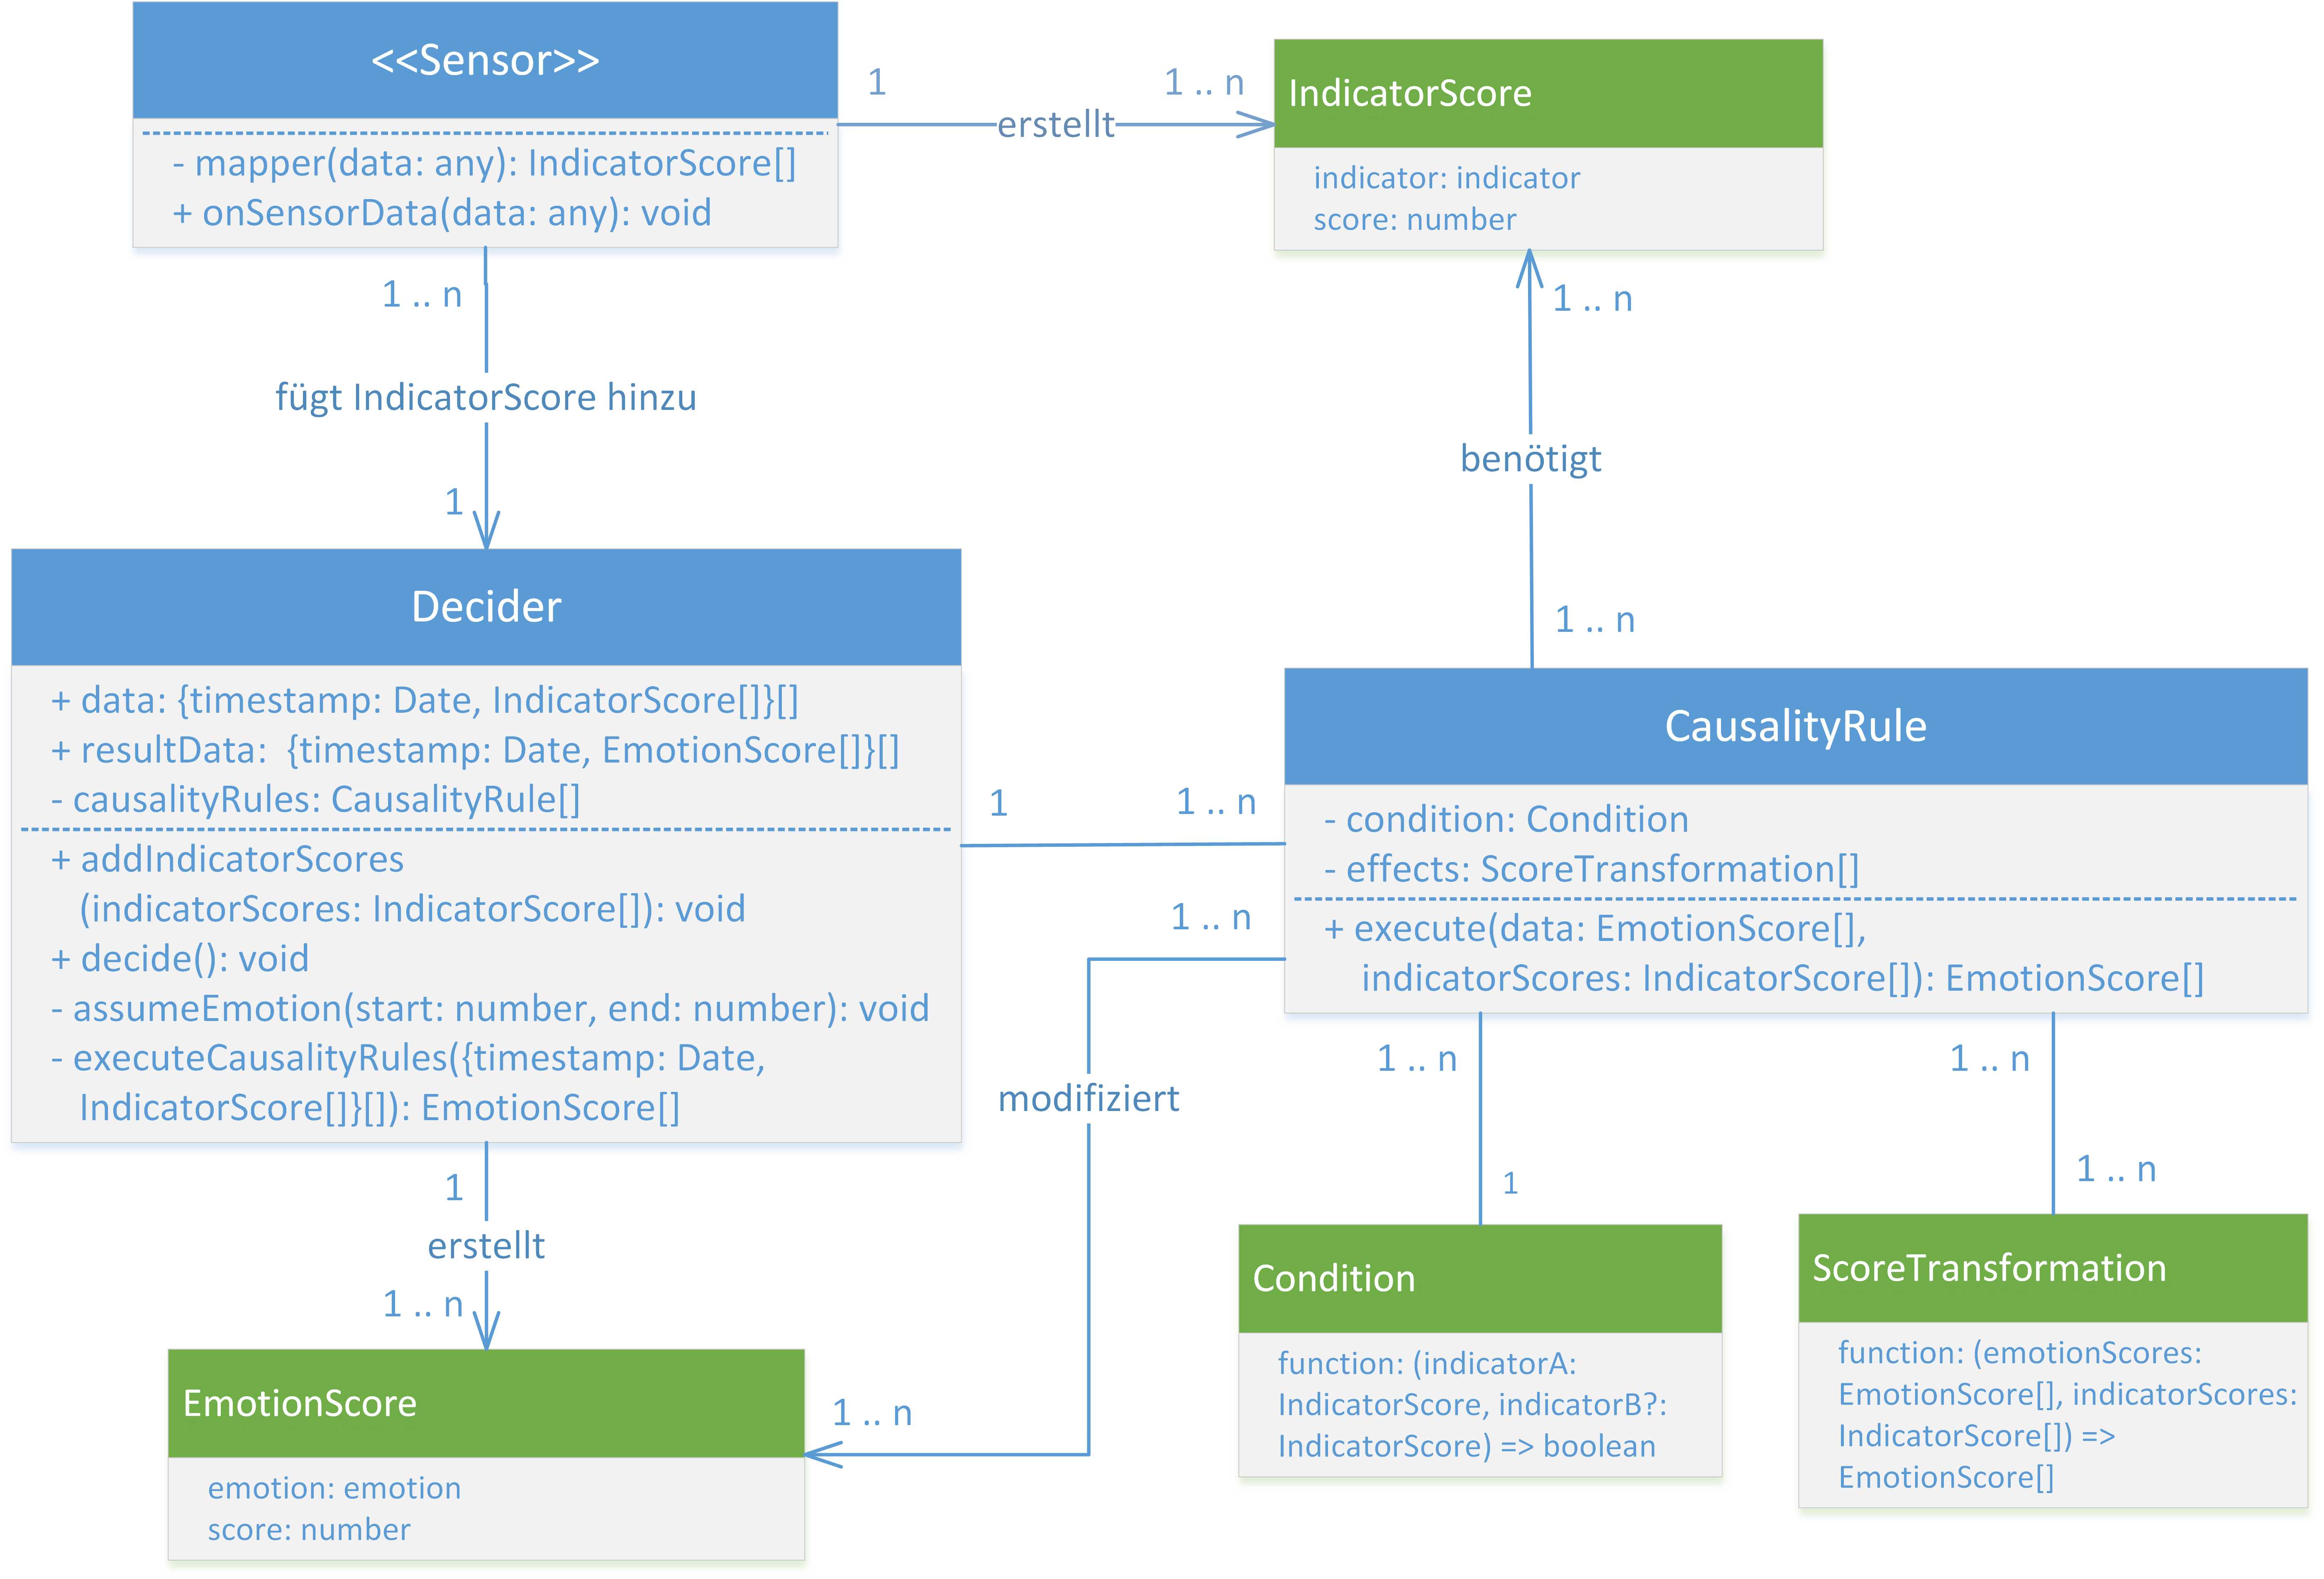
\includegraphics[width=16cm]{Bilder/architecture.png}
	\caption[Architektur der App]{Architektur der App}
\end{figure}%
Die Klassen sind in der Abbildung blau dargestellt. Typescript bietet die Möglichkeit, eigene Typen zu definieren. Diese Typen verfügen über Attribute, jedoch keine Methoden und sind in der Abbildung grün dargestellt. \newline \newline
Die App verfügt über eine abstrakte Klasse Sensor, die zwei Methoden definiert. Jeder Sensor, der später Daten für die App liefern soll, muss diese abstrakte Sensor-Klasse erweitern. Dabei muss jeder Sensor die mapper-Funktion überschreiben, die die Sensordaten in mehrere IndicatorScores umwandelt. Auf diese Weise muss jeder Sensor seinen individuellen Mapper implementieren. Der IndicatorScore ist als Typ definiert worden, der einerseits einen Indicator und einen Score als Attribut hat. Indicator wiederum ist ein eigener Typ, der nur die definierten Indikatoren (stress, happyIndicator, sadIndicator, angryIndicator, suprisedIndicator) als String zulässt. Da die Implementierung des IndicatorScore-Types sehr trivial ist, wurde sie aus Übersichtsgründen nicht in die Abbildung aufgenommen. Die onSensorData-Funktion ist bereits vordefiniert und muss dementsprechdend nicht überschrieben werden. Diese Funktion führt lediglich den Mapper aus, wenn genug Sensordaten für eine Auswertung vorhanden sind, und fügt die resultierenden IndicatorScores zum Decider hinzu. \newline \newline
Die Decider-Klasse ist der Hauptbestandteil der App, da sie die Bestimmung der Emotion durchführt. Die Decider-Klasse ist als Singleton anzusehen, da es pro laufende Aunwendung nur einen Decider geben kann. Der Decider verfügt über ein data-Array, das allen Input der Sensoren enthält. Konkret handelt es sich hierbei um die Indicatorscores, die die Sensoren ermittelt haben, erweitert mit einem Timestamp für den Zeitpunkt der Ankunft. Nach und nach wird dieses Array mit den IndicatorScores der verschiedenen Sensoren gefüllt. Dies wird mit der Funktion addIndicatorScores() realisiert, die von den Sensoren mit der onSensorData-Funktioen aufgerufen wird. \newline
Der Decider verfügt außerdem über ein Array von CausalityRules. Die CausalityRule-Klasse ist die Implementierung der oben beschriebenen Kausalitätsregel. Eine CausalityRule besitzt immer eine Condition (Bedinung) und eine Menge von ScoreTransformationen. \newline
Eine Condition wurde als eigener Typ definiert und ist eine Funktionen, die einen  IndicatorScore (optional auch zwei) als Input hat und auf einen Boolean-Wert abbildet. So kann eine Bedingung realisiert werden, die je nach Erfüllung true oder false zurückgibt. Eine ScoreTransformation ist ebenfalls ein eigener Typ, der eine Funktion definiert. Diese Funktion erhält als Input die vorhandenen Emotionscores, wendet auf diesen Effekte an und gibt die modifizierten Emotionscores zurück. \newline
Die execute-Funktion der CausalityRule führt alle hinterlegten ScoreTransformations aus, wenn die Condition von den IndicatorScores erfüllt worden ist. \newline
Um die Decider-Klasse weiter zu verstehen, muss zunächst der Typ Emotionscore erklärt werden. Dieser ist ähnlich wie der IndicatorScore aufgebaut. Zunächst wird eine Emotion angegeben, die dem Typ Emotion entsprechen muss. Der String muss dementsprechend mit den definierten Emotionen (happy, sad, angry, suprised) übereinstimmen. Anschließend folgt eine Nummer, die den Score angibt.\newline \newline
Die Decider hat ein resultData-Array, das mehrere Emotionscores enthält und die Timestamp der IndicatorScores, aus denen die Emotionscores erzeugt wurden. Dieses Array wird mithilfe der decide-Funktion gefüllt. Wenn die decide-Funktion ausgeführt wird, wird anschließend für alle im data-Array vorhandenen Timestamps die assumeEmotion()-Funktion ausgeführt. Als Parameter erhält diese Methode eine Timestamp und filtert alle IndicatorScores aus dem data-Array zu diesem Zeitpunkt. Für alle auf diese Weise gefilterten Indicatorscores wird anschließend die executeCausalityRules()-Funktion ausgeführt. Diese Funktion wiederum iteriert über alle vorhandenen CausalityRules und führt diese auf Basis der IndicatorScores aus. So erhält man am Ende Emotionscores. Diese erhalten die Timestamp, die bei assumeEmotion() mitgegeben wurde und werden in das resultData-Array gespeichert. Hat man die assumeEmotion-Funktion für alle Timestamps ausgeführt, ist das result-Array komplett gefüllt und die Emotionsbestimmung abgeschlossen.
\subsubsection{Frontend}
Nachdem bereits das Backend beschrieben wurde, wird nun das Frontend der App thematisiert. Unter dem Frontend werden die Screens der App verstanden, die der User bei Nutzung der App aufrufen kann. Diese Screens werden bei Ionic Pages genannt und bestehen meist aus folgenden Bestandteilen: 
\begin{itemize}[noitemsep, topsep=0pt]
	\item Eine Typescript-Datei (.ts), 
	\item eine HTML-Datei (.html) und
	\item eine CSS-Datei (.scss).
\end{itemize}
In der Typescript-Datei wird die Anwendungslogik umgesetzt, außerdem erfolgt dort der Zugriff auf die Backendkomponenten wie zum Beispiel den Decider, die durch das Ionic Framework als sogenannte Provider bereitgestellt werden. Die HTML-Datei beschreibt den Aufbau der GUI der Page, wohingegen die CSS-Datei das Design der Page beschreibt. \newline
In Abbildung ? ist zu sehen, über welche Pages die App verfügen soll, welchen Zweck diese haben und wie sie miteinander in Verbindung stehen.
\begin{figure}[h]
	\centering
	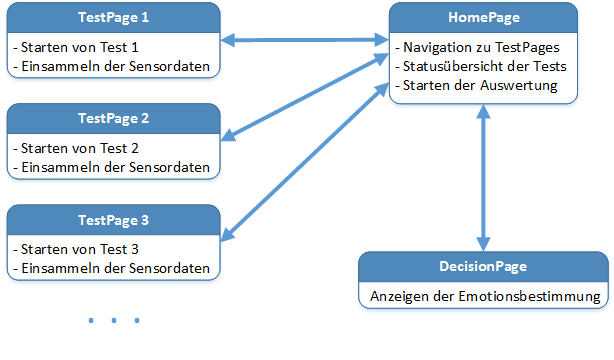
\includegraphics[width=15cm]{Bilder/frontend.png}
	\caption[Geplantes Frontend der App]{Geplantes Frontend der App}
\end{figure}% 
\newline
Für die App sollen nach und nach sogenannte Emotionstest entwickelt werden. Unter einem Emotionstest versteht man im Kontext dieses Projekts die Messung eines Sensors, die Rückschlüsse auf die Emotion zulassen. Ein Emotionstest liefert aus Backend-Sicht immer eine Menge von Indikatorscores zurück. Pro Emotionstest muss eine Page der App angelegt werden, auf der der Test gestartet werden kann und so die Sensormessdaten eingesammelt werden können. \newline
Zwangsläufig verfügt die App über eine HomePage, auf die der User beim Starten der App gelangt. Über diesen Screen kann der User zu den einzelnen TestPages gelangen, um die Tests durchzuführen. Von den TestPages kann der User entweder durch Abschließen der Tests oder durch manuelles Navigieren und Unterbrechen des Test zurück zum Homescreen gelangen. Um dem User anzuzeigen, welche Test er schon durchgeführt hat, wird außerdem eine Statusübersicht zu den Tests auf der HomePage zu sehen sein. Des Weiteren muss der User die Möglichkeit haben, die Auswertung der Indicatorscores zu Emotionen starten zu können. Wählt der User diese Option, werden alle Indicatorscores, die sich zu diesem Zeitpunkt im data-Array des Deciders befinden für die Auswertung verwendet. \newline
Für das Ergebnis der Auswertung und somit die Emotionsbestimmung muss ebenfalls eine eigene Page existieren, worauf der User nach Abschluss der Auswertung gelangt. Der User kann von diesem Screen wieder zurück zum Homescreen gelangen, um erneut Emotionstests zu starten.  